\chapter{Different Reset schemes and their expectations}

\section{Pumping Reset Scheme}
\subsection{Intuition behind scheme}



\section{Master Equation Formalism}
The crux of the quantum information processing is to understand the sources of the dissipation for possible remedies. However, the complexity of the interaction between the quantum system of interest and the surrounding environment render a general and assumption-free analysis intractable. In the closed system point of view, the result of the interaction between system and environment is a non-unitary evolution of the system's degrees of freedom, whose evolution can be modelled with stochastic wavefunction description \cite{smqo1}. In this description, the wavefunction of the system discovers one one the possible trajectories in its phase space, which is corresponding what could be observed in a single experimental run. As its name suggesting, this process is a non-deterministic process in which no deterministic control can be established over.

\vspace{2 mm}

On the other hand, under certain assumptions, the evolution of the closed system can be described by master equations \cite{davies}. In usual cases, the number of degrees of freedom in environment is huge such that the information leaked from the close system to environment cannot flow back to the system in any finite time, i.e. whenever the environment interacts with the closed system, the obtained information is quickly forgotten by the environment  due very short self-correlation time \cite{ahn}. Furthermore, if the environment (or reservoir) is considered as a measurement device which continuously probes the closed system, the resulting dynamics can be described as an average realization of each possible individual trajectories in the phase space of the total system. Alongside with this, the interaction between the closed system and environment is weak, and further separability of density functions of closed system and environment, the overall dynamics of the system can be described by Lindblad master equation formalism\footnote{The intricacies of the derivation leading to Lindblad master equation will not be discussed in the remainder of the report; however, for more detailed analysis can be found in the seminal work of C.W. Gardiner and M.J Collett \cite{gardinercollet1985}, and also "Theory of quantum noise and decoherence" course of Tobias J. Osborne in Youtube.}: 

\begin{equation}
    \Dot{\rho} = -i[H,\rho] + \sum_{\i=1}^{m} \mathcal{D}[c_i]\pho
\end{equation}

where the Lindblad superoperator $\mathcal{D}$ is $\mathcal{D}[c]\rho = c\rho c^\dagger - \frac{1}{2}c^\dagger c \rho -\frac{1}{2} \rho c^\dagger c$, and $\rho$ is the density matrix of the closed system (i.e. the density matrix obtained after the reservoir is traced out).

Thus, to be able to see the evolution of the closed system's density, the Hamiltonian of the system, the form of the collapse operators regarding the various dissipation or decoherence channels and the initial condition of the density matrix are the only requirements. In the next section, the question regarding on how to simulate the system will be explained in the pumping reset scheme specific.


\section{Master Equation Simulation of Pumping Reset Scheme with QuTiP }

\maketitle
	
\subsection{Hamiltonian}

	\begin{equation} \label{eq:full_hamiltonian}
	\begin{split}
		H = \underbrace{\hbar \omega_{eg}b^\dagger b - \frac{\alpha}{2} b^\dagger b ^\dagger b b }_{\text{qubit hamiltonian}}+ \underbrace{\hbar \omega_{1} a ^ \dagger a}_{\text{cavity mode}} + \underbrace{\hbar \omega_{2} c ^\dagger c}_{\text{reset mode}} + \underbrace{\hbar \omega_{3} d ^\dagger d}_{\text{pump mode}} \\
		+\underbrace{\hbar  g_1(b^\dagger a + a ^\dagger b) + \hbar g_2(b^\dagger c + c^\dagger b) + \hbar g_3(b^\dagger d + d^\dagger b)}_{\text{interaction term}}.
    \end{split}
	\end{equation}

	By choosing this form of the Hamiltonian, the rotating wave approximation is already applied. On the other hand, the time dependence of the interaction term was not written explicitly in Eqn. \ref{eq:full_hamiltonian}. For the rest of the analysis, the Hamiltonian is parted into two parts, namely quadratic and quartic.
	
\vspace{3mm}

	Now we write down the quadratic term,
	\begin{equation} \label{eq:h2}
	\begin{split}
		h_2 = \hbar \omega_{eg}b^\dagger b + \hbar \omega_{1} a ^ \dagger a +\hbar \omega_{2} c ^\dagger c + \hbar \omega_{3} d ^\dagger d \\
		+\hbar  g_1(b^\dagger a + a ^\dagger b) + \hbar g_2(b^\dagger c + c^\dagger b) + \hbar g_3(b^\dagger d + d^\dagger b) 
    \end{split}
	\end{equation} 
	
	And quartic term of the Hamiltonian,
	
	\begin{equation}\label{eq:h4}
	h_4 =- \frac{\hbar \alpha}{2} b^\dagger b ^\dagger b b 
	\end{equation}

	It can be better illustrated if we display $h_2$ in matrix format,
	\begin{equation}
		\frac{h_2}{\hbar} = \begin{pmatrix} b^\dagger & a ^ \dagger & c^\dagger & d^\dagger \end{pmatrix}
		\begin{pmatrix}
		\omega_{ge} & g_1 & g_2 & g_3 \\
		g_1 & \omega_1 & 0 & 0 \\
		g_2 & 0 & \omega_2 & 0\\
		g_3 & 0 & 0& \omega_3
		\end{pmatrix}
		\begin{pmatrix} b \\ a \\ c  \\ d\end{pmatrix}
	\end{equation}


	To diagonalize $h_2$ we would like to calculate eigenvectors of the coefficient matrix. However, the root of a qubic equation is usually complicated, which leads to even more complex expression of eigenvectors. However, the detuning between the modes and the values of the coupling strengths allow neglecting the complicated higher order terms in the perturbative approach.

	Define the parameters
	\begin{equation}
		\begin{cases}
			\Delta_1 = \omega_1 - \omega_{ge} \\
			\Delta_2 = \omega_2 - \omega_{ge} \\
			\Delta_3 = \omega_3 - \omega_{ge} \\
			\varepsilon_1 = g_1 / \Delta_1 \\
			\varepsilon_2 = g_2 / \Delta_2 \\
			\varepsilon_3 = g_3 / \Delta_3
		\end{cases}
	\end{equation}

	First-order correction to eigenvectors are
	\begin{equation} \label{eq:1st-order-correction}
		\Phi_i^1 = \sum _{j \neq i} \frac{\langle \Phi_j | V | \Phi_i \rangle}{E_j - E_i}
	\end{equation}

In this case, ${E_i}$ denotes diagonal elements of coefficient matrix, while ${V_{ij}}$ denotes off-diagonal elements. Substituting first-order correction to Eq\ref{eq:1st-order-correction}, we obtain new eigenvectors
\begin{equation}
	\begin{cases}
		\tilde{b} = b - \frac{g_1}{\Delta_1} a - \frac{g_2}{\Delta_2} c - \frac{g_3}{\Delta_3} d \\
		\tilde{a} = a + \frac{g_1}{\Delta_1} b \\
		\tilde{c} = c + \frac{g_2}{\Delta_2} b \\
		\tilde{d} = d + \frac{g_3}{\Delta_3} b
	\end{cases}
\end{equation}

Inverse the solution and we will get the first order correction on diagonalizing $h_2$
\begin{equation} \label{eq:diagonalize}
	\begin{cases}
		b = \tilde{b} + \frac{g_1}{\Delta_1} \tilde{a} + \frac{g_2}{\Delta_2} \tilde{c} +\frac{g_3}{\Delta_3} \tilde{d} \\
		a = \tilde{a} - \frac{g_1}{\Delta_1} \tilde{b} \\
		c = \tilde{c} - \frac{g_2}{\Delta_2} \tilde{b} \\
		d = \tilde{d} - \frac{g_3}{\Delta_3} \tilde{b}
	\end{cases}
\end{equation}

The substitution given in Eqn. \ref{eq:diagonalize} diagonalizes $h_2$ by cancelling the direct interaction term between the cavity modes and qubit mode and producing terms in $\mathcal{O}(\frac{g^2}{\Delta^2})$, which are negligible in the weak coupling and/or large detuning.  After the substitution, the quadratic part of the Hamiltonian becomes, 

\begin{equation} \label{eq:h2_bare_tilde}
    \frac{h_{2,bare}}{\hbar} = (\omega_{eg}-\frac{g_1^2}{\Delta_1}-\frac{g_2^2}{\Delta_2}-\frac{g_3^2}{\Delta_3})\tilde{b}^\dagger \tilde{b} + (\omega_1+\frac{g_1^2}{\Delta_1})\tilde{a}^\dagger \tilde{a}+ (\omega_2+\frac{g_2^2}{\Delta_2})\tilde{c}^\dagger \tilde{c} + (\omega_3+\frac{g_3^2}{\Delta_3})\tilde{d}^\dagger \tilde{d}
\end{equation}

In addition to terms in Eqn. \ref{eq:h2_bare_tilde}, this substitution introduces effective interaction term between readout and reset resonator and also effective driving terms for both resonators, which are mediated by qubit,

\begin{equation} \label{eq:h2_int_tilde}
    \frac{h_{2,int}}{\hbar} = \omega_{eg} \frac{g_1 g_2}{\Delta_1 \Delta_2}(\tilde{a}^\dagger \tilde{c} + \tilde{a} \tilde{c}^\dagger) + \omega_{eg} \frac{g_2 g_3}{\Delta_2 \Delta_3}(\tilde{c}^\dagger \tilde{d} + \tilde{c} \tilde{d}^\dagger) +\omega_{eg} \frac{g_1 g_3}{\Delta_1 \Delta_3}(\tilde{a}^\dagger \tilde{d} + \tilde{a} \tilde{d}^\dagger)
\end{equation}
Although the terms in Eqn. \ref{eq:h2_int_tilde} are rotating fast with compared to the timescale of interest, their coefficients are significant enough to affect the fidelity of reset process. Thus, they are taken into account in Lindblad master eqaution simulation. Next, we would like to substitute the corresponding terms in $h_4$ in order to get the corrections on state-depending frequency shift and two-photon process.

\begin{equation} \label{eq:h4-correction}
    \frac{h_4}{\hbar} = -\frac{\alpha}{2} (\tilde{b}^\dagger + \varepsilon_1 \tilde{a}^\dagger + \varepsilon_2 \tilde{c}^\dagger + \varepsilon_3 \tilde{d}^\dagger)^2 (\tilde{b} + \varepsilon_1 \tilde{a} + \varepsilon_2 \tilde{c} + \varepsilon_3 \tilde{d})^2
\end{equation}

The expansion of the Eqn. \ref{eq:h4-correction} contains 64 terms. After rotating wave approximation, considering the pumping mode as a coherent EM tone and ignoring the terms having the coefficient proportional to $\epsilon^3$ or higher, the number of terms in the quartic Hamiltonian is significantly reduced. First, let's focus on the terms corresponding to frequency shifts occurring qubit's transition frequency due to the EM modes coupled dispersively\footnote{Mode operators with tilde are written without tilde (i.e. $\tilde{O} \xrightarrow[]{} O$) to simplify the notation.},

\begin{equation} \begin{split}
	\chi_1 &= -2\alpha \varepsilon_1^2 b^\dagger b a^\dagger a \\
	\chi_2 &= -2\alpha \varepsilon_2^2 b^\dagger b c^\dagger c \\
	\chi_3 &= -2\alpha \varepsilon_3^2 \abs{\Omega_d}^2 b^\dagger b 
\end{split} \end{equation}

This corresponds to dispersive shift due to coupling between qubit and two quantized modes (the modes of readout and reset resonator), and one coherent EM field (pump mode). As we have already explained in the introduction, an effective two photon process can be engineered by choosing the frequency of the coherent field as,

\begin{equation} \begin{split}
 \omega_3 = \omega_2 - 2\tilde{\omega}_{eg} + \alpha 
\end{split} \end{equation}

where $\tilde{\omega}_{eg}$ is the renormalized transition frequency of the qubit after the effects of other modes are taken into account. Consequently, 
\begin{equation}
	H_{2-pho} = -\alpha\varepsilon_2\varepsilon_3(b^\dagger b^\dagger cd+bbc^\dagger d^\dagger)
\end{equation}

This term corresponds to two-photon interaction between qubit, resonator field and pump field. If we pump with coherent light field, we can substitute operator $d$ by $\Omega_d$ (assume $\Omega_d$ to be real).
\begin{equation}
	H_{2-pho} = -\alpha\varepsilon_2\varepsilon_3\abs{\Omega_d} (b^\dagger b^\dagger c e^{i\omega_3 t} + bbc^\dagger e^{-i\omega_3 t})
\end{equation}

The coefficient $\alpha\varepsilon_2\varepsilon_3\Omega_d$ represents the rate of this two-photon process. Since, the coefficients $\varepsilon_2$ and $\varepsilon_3$ are small numbers due to detuning, the drive strength should be high in order to observe the effect of the two-photon process, which is needed to pump the population in $\ket{f}$ level of the qubit to lossy cavity mode ($\hat{c}$). The other important term is the effective driving of the qubit by the pump mode ($\hat{d}$) due to its amplitude,

\begin{equation}
	H_{ind,dri} = -\alpha (2\varepsilon_3 b^\dagger b \abs{\Omega_d} + \varepsilon_3^3 \abs{\Omega_d}^3) (b^\dagger e^{i\omega_3 t} +b e^{-i \omega_3 t})
\end{equation}

As a result, the Hamiltonian of the system after the perturbative approach, 

\begin{equation}\begin{split}
   \frac{\mathcal{H}}{\hbar} = (\omega_{eg}-\frac{g_1^2}{\Delta_1}-\frac{g_2^2}{\Delta_2}-\frac{g_3^2}{\Delta_3})b^\dagger b + (\omega_1+\frac{g_1^2}{\Delta_1})a^\dagger a+ (\omega_2+\frac{g_2^2}{\Delta_2})c^\dagger c  \\
\omega_{eg} \frac{g_1 g_2}{\Delta_1 \Delta_2}(a^\dagger c + a c^\dagger) + \omega_{eg} \frac{g_2 g_3}{\Delta_2 \Delta_3}\abs{\Omega_d}(c^\dagger e^{i\omega_3 t} + c e^{-i\omega_3 t}) +\omega_{eg} \frac{g_1 g_3}{\Delta_1 \Delta_3}\abs{\Omega_d}(a^\dagger e^{i\omega_3 t}+ a e^{-i\omega_3 t}) \\
  -2\alpha \varepsilon_1^2 b^\dagger b a^\dagger a 
	 -2\alpha \varepsilon_2^2 b^\dagger b c^\dagger c 
	 -2\alpha \varepsilon_3^2 \abs{\Omega_d}^2 b^\dagger b \\
-\alpha\varepsilon_2\varepsilon_3\abs{\Omega_d} (b^\dagger b^\dagger c e^{i\omega_3 t} + bbc^\dagger e^{-i\omega_3 t})\\
-\alpha (2\varepsilon_3 b^\dagger b \abs{\Omega_d} + \varepsilon_3^3 \abs{\Omega_d}^3) (b^\dagger e^{i\omega_3 t} +b e^{-i \omega_3 t})
\end{split}
\end{equation}

\subsection{Collapse Operators}

In this section, the interaction between the close system comprised of qubit-cavity and the environment. In our system, the following decoherence and dissipation sources are taken into account:

\begin{itemize}
  \item Decay rate of the readout resonator: $\kappa_{read}$
  \item Decay rate of the reset resonator: $\kappa_{reset}$
  \item Decay rate of transmon in between $\ket{g}$ and $\ket{e}$: $\gamma_{1,ge}$
  \item Decay rate of transmon in between $\ket{e}$ and $\ket{f}$: $\gamma_{1,ef}$
  \item Pure dephasing rate of transmon in between $\ket{g}$ and $\ket{e}$: $\gamma_{\phi,ge}$
  \item Pure dephasing rate of transmon in between $\ket{e}$ and $\ket{f}$: $\gamma_{\phi,ef}$
\end{itemize}


\subsection{Form of the Master Equation}

As a result, the final form of the master equation becomes,

\begin{equation} \begin{split}
	\Dot{\rho} = -i[\hat{\mathcal{H}},\rho] + \kappa_{read}\mathcal{D}[\hat{a}]\rho +  \kappa_{reset}\mathcal{D}[\hat{c}]\rho  \\
	+(n_{th}+1)\gamma_{1,ge}\mathcal{D}[\ket{g}\bra{e}]\rho + n_{th} \gamma_{1,ge}\mathcal{D}[\ket{e}\bra{g}]\rho\\
	+\gamma_{1,ef}\mathcal{D}[\ket{e}\bra{f}]\rho  + n_{th} \gamma_{1,ef}\mathcal{D}[\ket{f}\bra{e}]\rho \\
	+ \frac{\gamma_{\phi,ge}}{2} \mathcal{D}[\ket{e}\bra{e}-\ket{g}\bra{g}]\rho + \frac{\gamma_{\phi,ef}}{2} \mathcal{D}[\ket{f}\bra{f}-\ket{e}\bra{e}]\rho
	\end{split}
\end{equation}

where $\mathcal{D}[\hat{O}] \bullet = \hat{O} \bullet \hat{O}^\dagger - \frac{1}{2}\left\{\hat{O}^\dagger \hat{O}, \bullet \right\}$ is the dissipation or decoherence superoperator, and $n_{th}$ is the thermal population of the transmon qubit in steady state. 

\section{QuTiP Simulation}

In this section, the simulation results of the Lindblad master equation for the Hamiltonian and collapse operators associated with the pumping reset scheme. In this simulation, we are considering the 7.4 GHz mode as the readout mode, and 18.75 GHz mode as the reset mode. The coupling strength between these modes and qubit are determined with the ANSYS simulations. On the other side, the qubit-related parameters are taken from Magnard et. al paper \cite{Magnard} given the fact that the design and fabrication of the qubit was cancelled due COVID-19 pandemic. 

\vspace{2 mm}

In this reset scheme, unlike Magnard et.al's approach, the pulse between $\ket{e}$ and $\ket{f}$ is a mere $\pi$-pulse without any optimization. The only control and optimization knob of this scheme is the duration and the frequency of the pumping pulse. Furthermore, since the frequency difference between $\ket{g,1}$ and  $\ket{f,0}$ states are depending on the pump frequency and pulse strength, it is analytically challenging to find the correct pulse parameters. Therefore, the first simulation aims to determine the frequency of the pumping pulse for a fixed pulse duration (150 ns) which yields the best reset fidelity, 

\begin{figure}[h]
    \centering
    \includegraphics[width=1\textwidth]{pic/different_reset_schemes/qubit_pop_max_reset_pop_to_det_freq.eps}
    \caption{a) The population of the qubit and b) the maximum value of the population of the reset resonator after the system is driven by 150 ns pulse with different frequencies.}
    \label{fig:freq_sweep_qubit_reset_max}
\end{figure}


\begin{figure}[h]
    \centering
    \includegraphics[width=1\textwidth]{pic/different_reset_schemes/gef_pop.eps}
    \caption{The population in $\ket{g}$, $\ket{e}$ and $\ket{f}$ state after the system is driven by 150 ns pulse with different frequencies.}
    \label{fig:freq_sweep_gef}
\end{figure}


In the first subplot in Fig. \ref{fig:freq_sweep_qubit_reset_max}, where the overall qubit population is depicted, the population is plummeting down near to zero for the frequency of 7.10 GHz, while the population in the reset resonator reaches its peak for this particular frequency, which signals that the population transfer from $\ket{f,0}$ to $\ket{g,1}$ is maximized. Furthermore in Fig. \ref{fig:freq_sweep_gef}, one can see that the population in $\ket{f}$ state is drained to $\ket{g}$ state but not to $\ket{e}$, which is evident from the fact that the population in $\ket{e}$ state is also attaining its lowest value.


\vspace{2 mm}

The next parameter to be simulated is the duration of the pulse. In the previous analysis, for a fixed pulse duration, which is 150 ns, the frequency difference between the states $\ket{f,0}$ and $\ket{g,1}$ was determined. However, the duration of the pulse is the other integral part of the Rabi flip between these states, since any trajectory on Bloch sphere is determined both frequency, coupling strength and duration of the driving term.  


For determining the pulse duration which yield near-perfect population transfer from the qubit subspace to reset resonator subspace, the population of the qubit states are investigated under different pulse durations ranging from 100 to 200 ns. In the simulations, the overall evolution time is set to 500 ns.



\begin{figure}[h!]
    \centering
    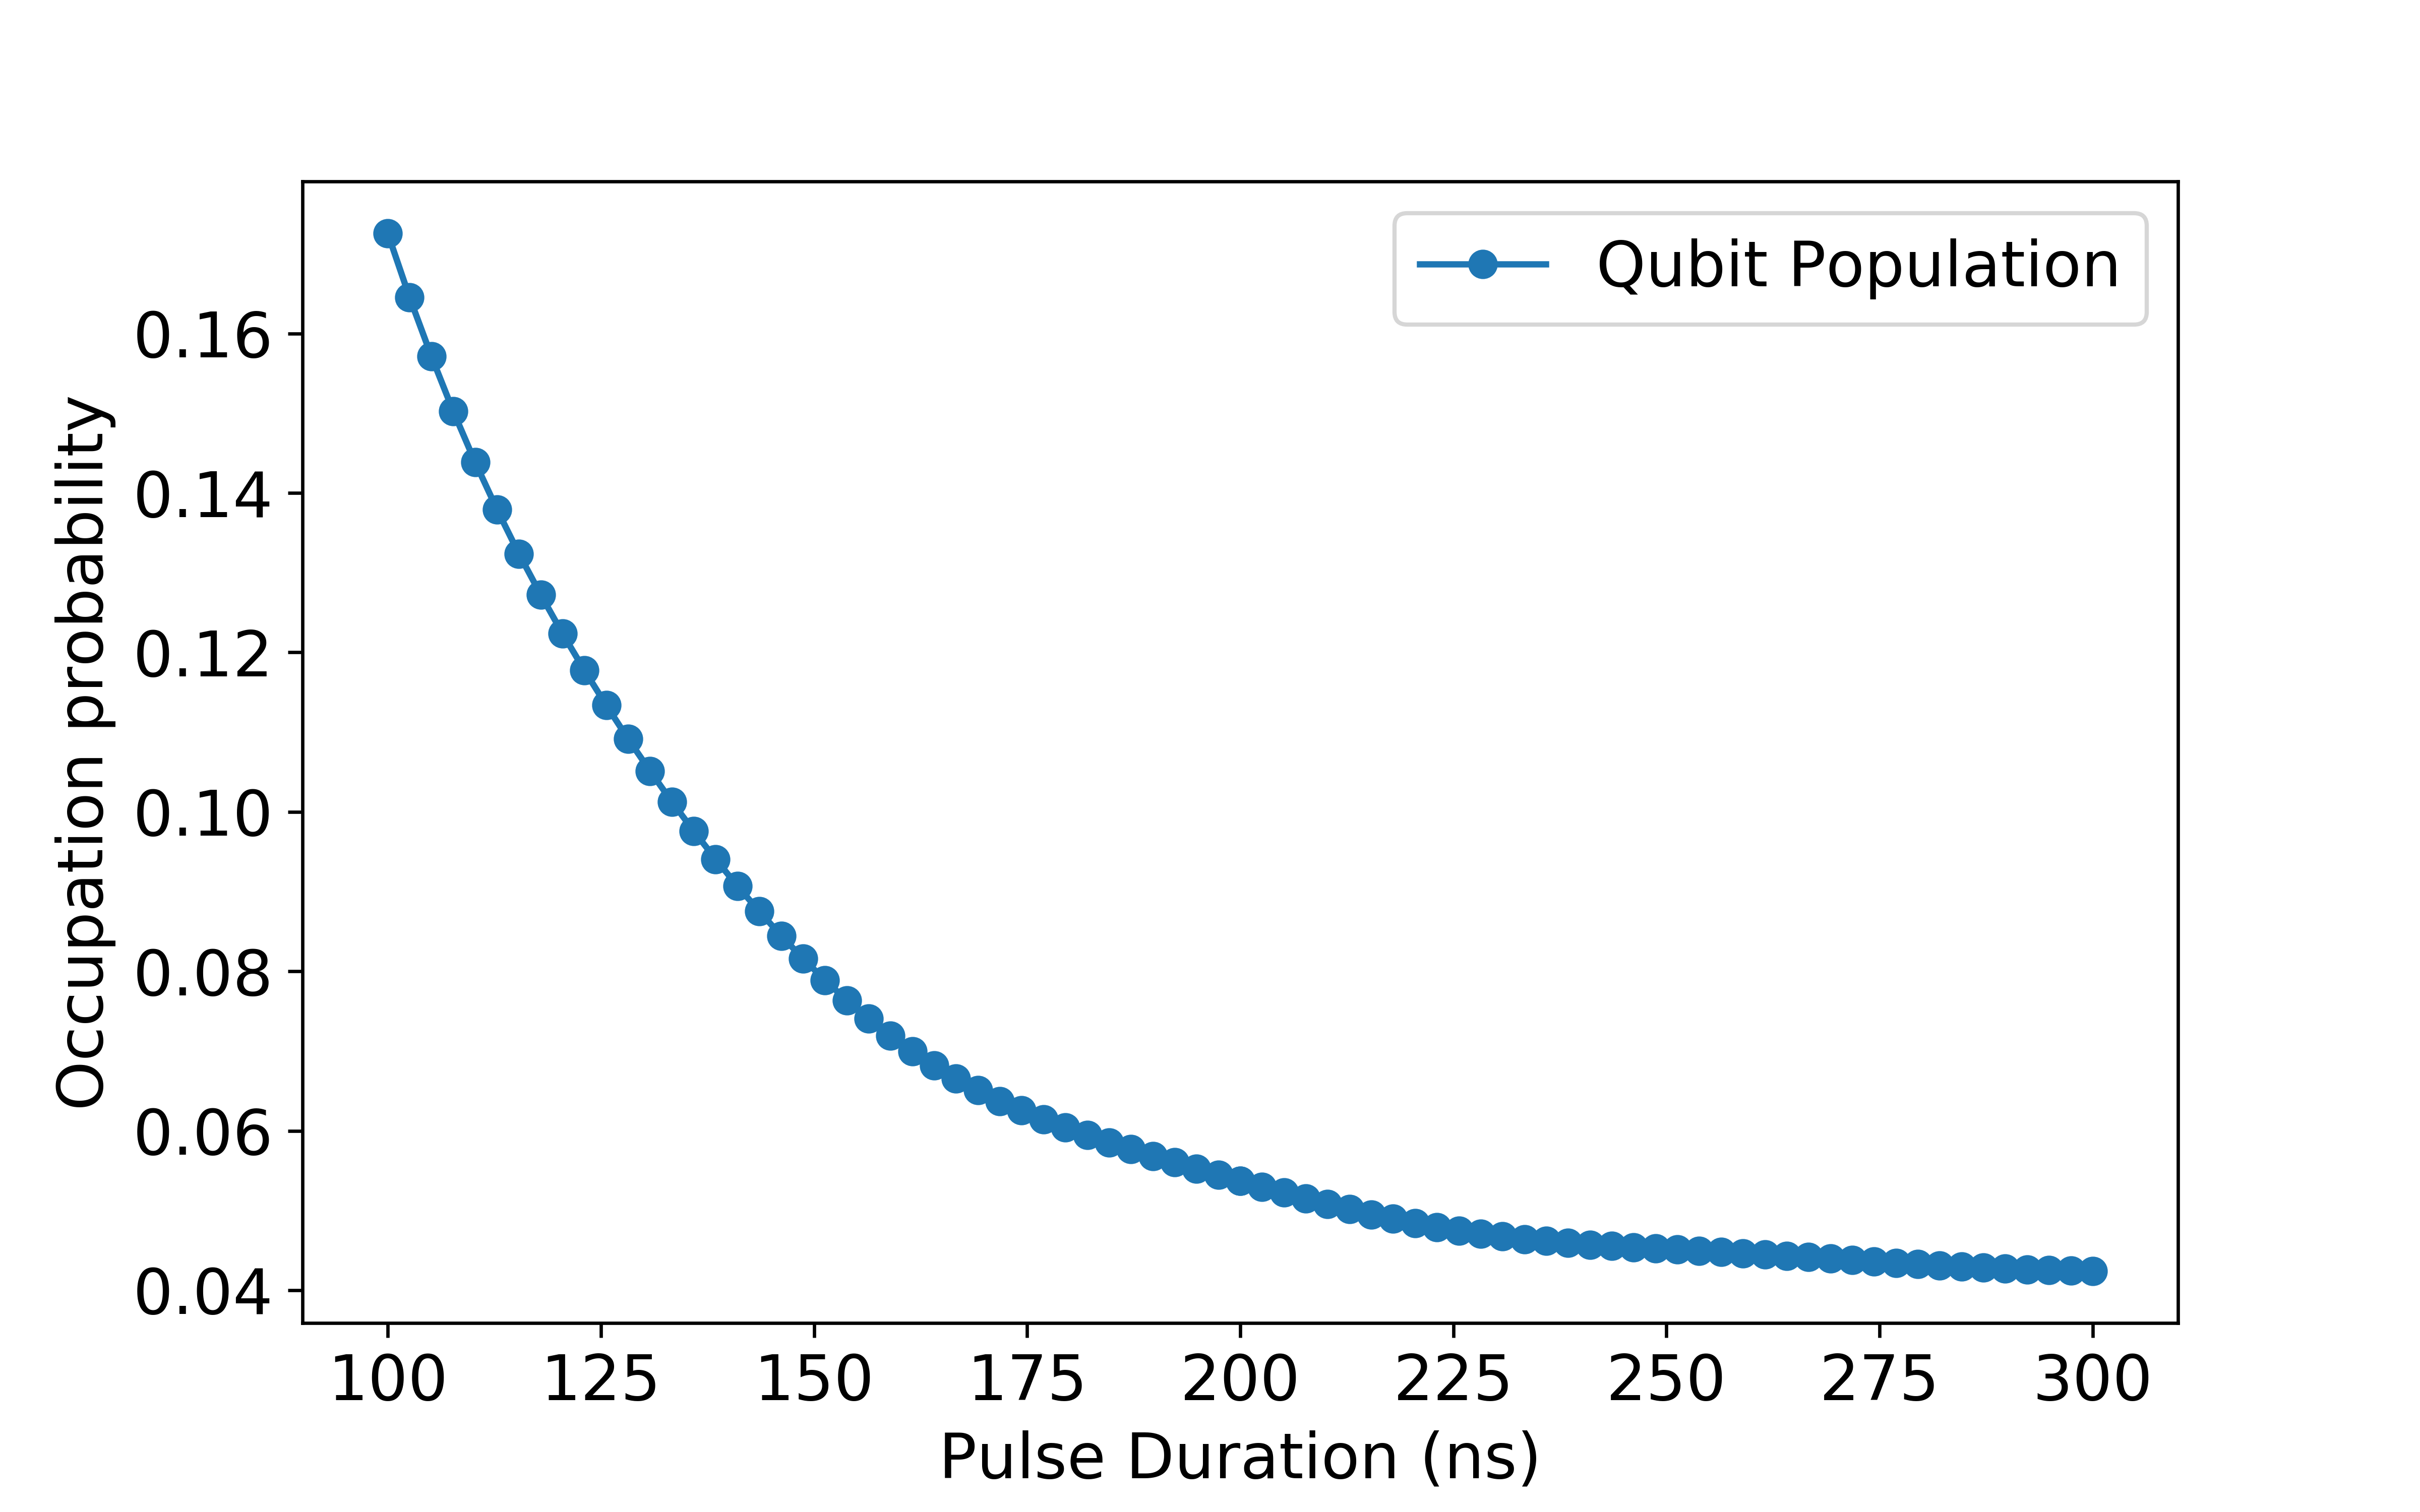
\includegraphics[width=0.6\textwidth]{pic/different_reset_schemes/qubit_pop_710_tau_sweep_100_300.png}
    \caption{The qubit and reset resonator population for pulse duration between 100 to 300 ns.}
    \label{fig:tau_sweep_qubit}
\end{figure}

\begin{figure}[h!]
    \centering
    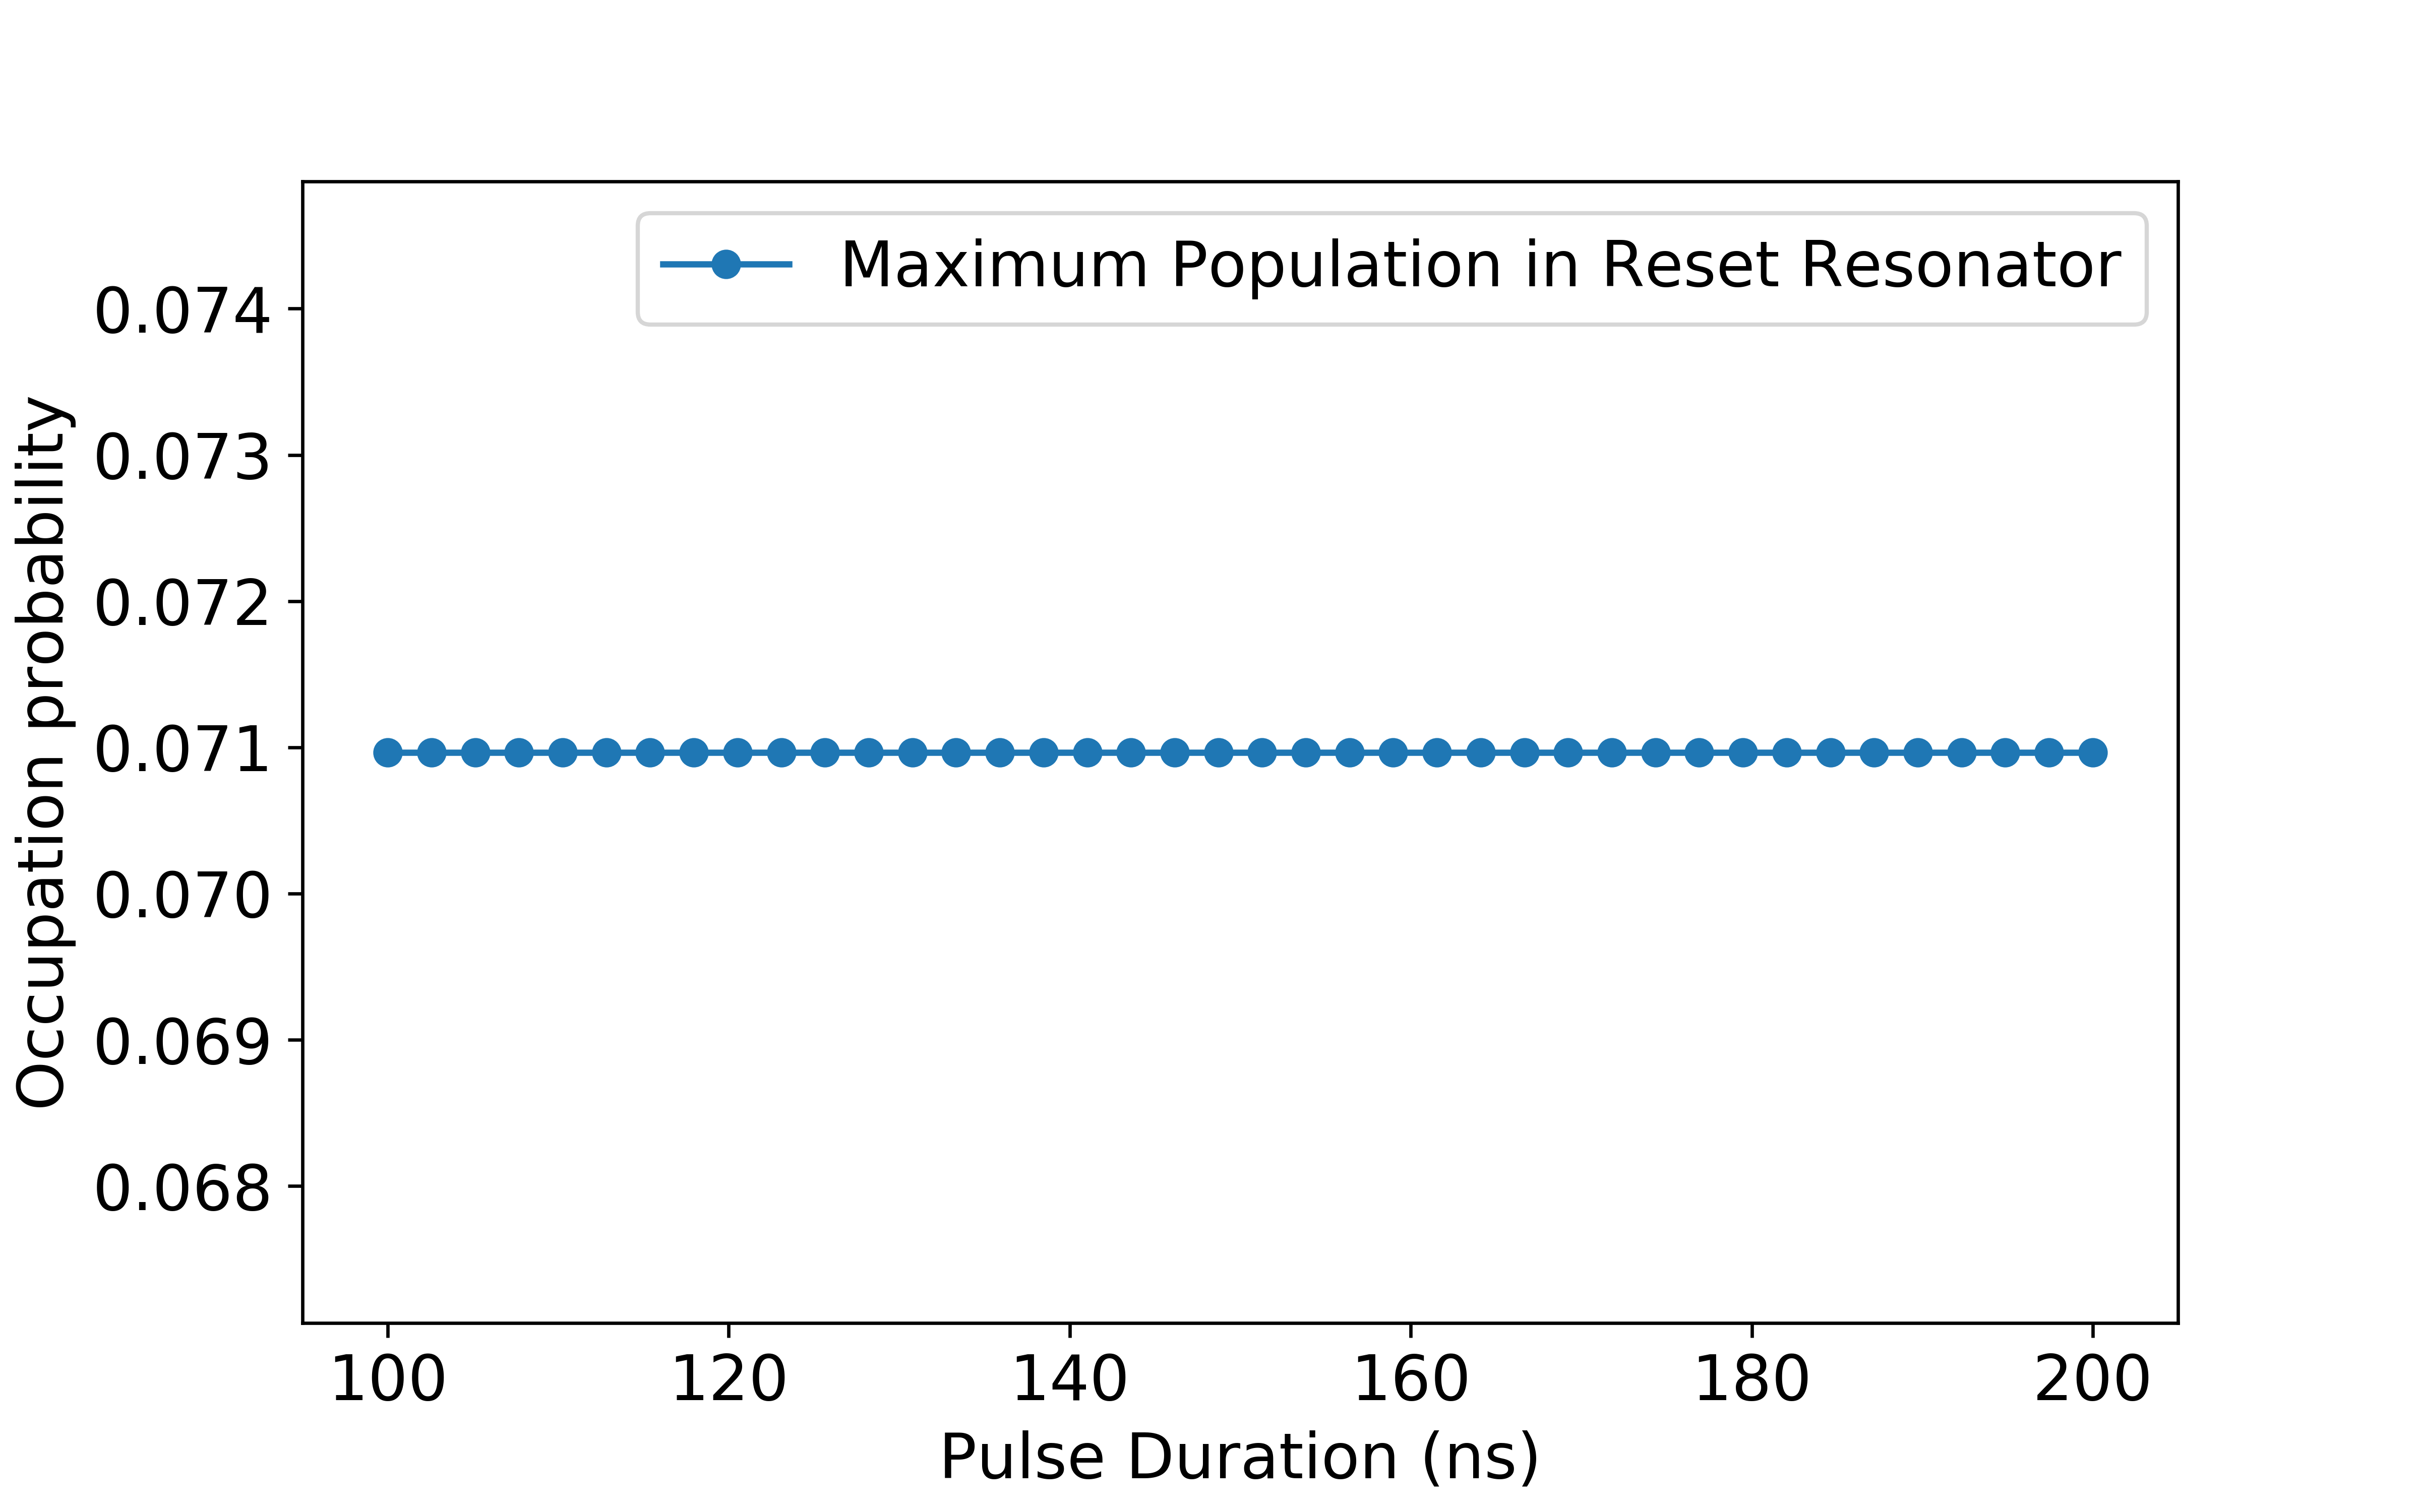
\includegraphics[width=0.6\textwidth]{pic/different_reset_schemes/reset_pop_max.png}
    \caption{The maximum value of the population of the reset resonator throughout its time evolution.}
    \label{fig:tau_sweep_reset}
\end{figure}


 While interpreting the plots in Fig. \ref{fig:tau_sweep_qubit}, the first thing that should be looked at the value of pulse duration where the population of reset resonator attains its maximum value. Since this duration signals the optimal duration of the driving pulse with specified frequency to realize a $\pi$-pulse between $\ket{f,0}$ and $\ket{g,1}$ states. In other words, higher the success of transferring the population from the qubit modes to reset modes, the faster and the more accurate reset operation. However, the population put into reset resonator is decayed too fast with compared to the Rabi timescale. Therefore, it is not possible to observe the signature of Rabi oscillation in Fig. \ref{fig:tau_sweep_qubit}. 



\begin{figure}[h!]
    \centering
    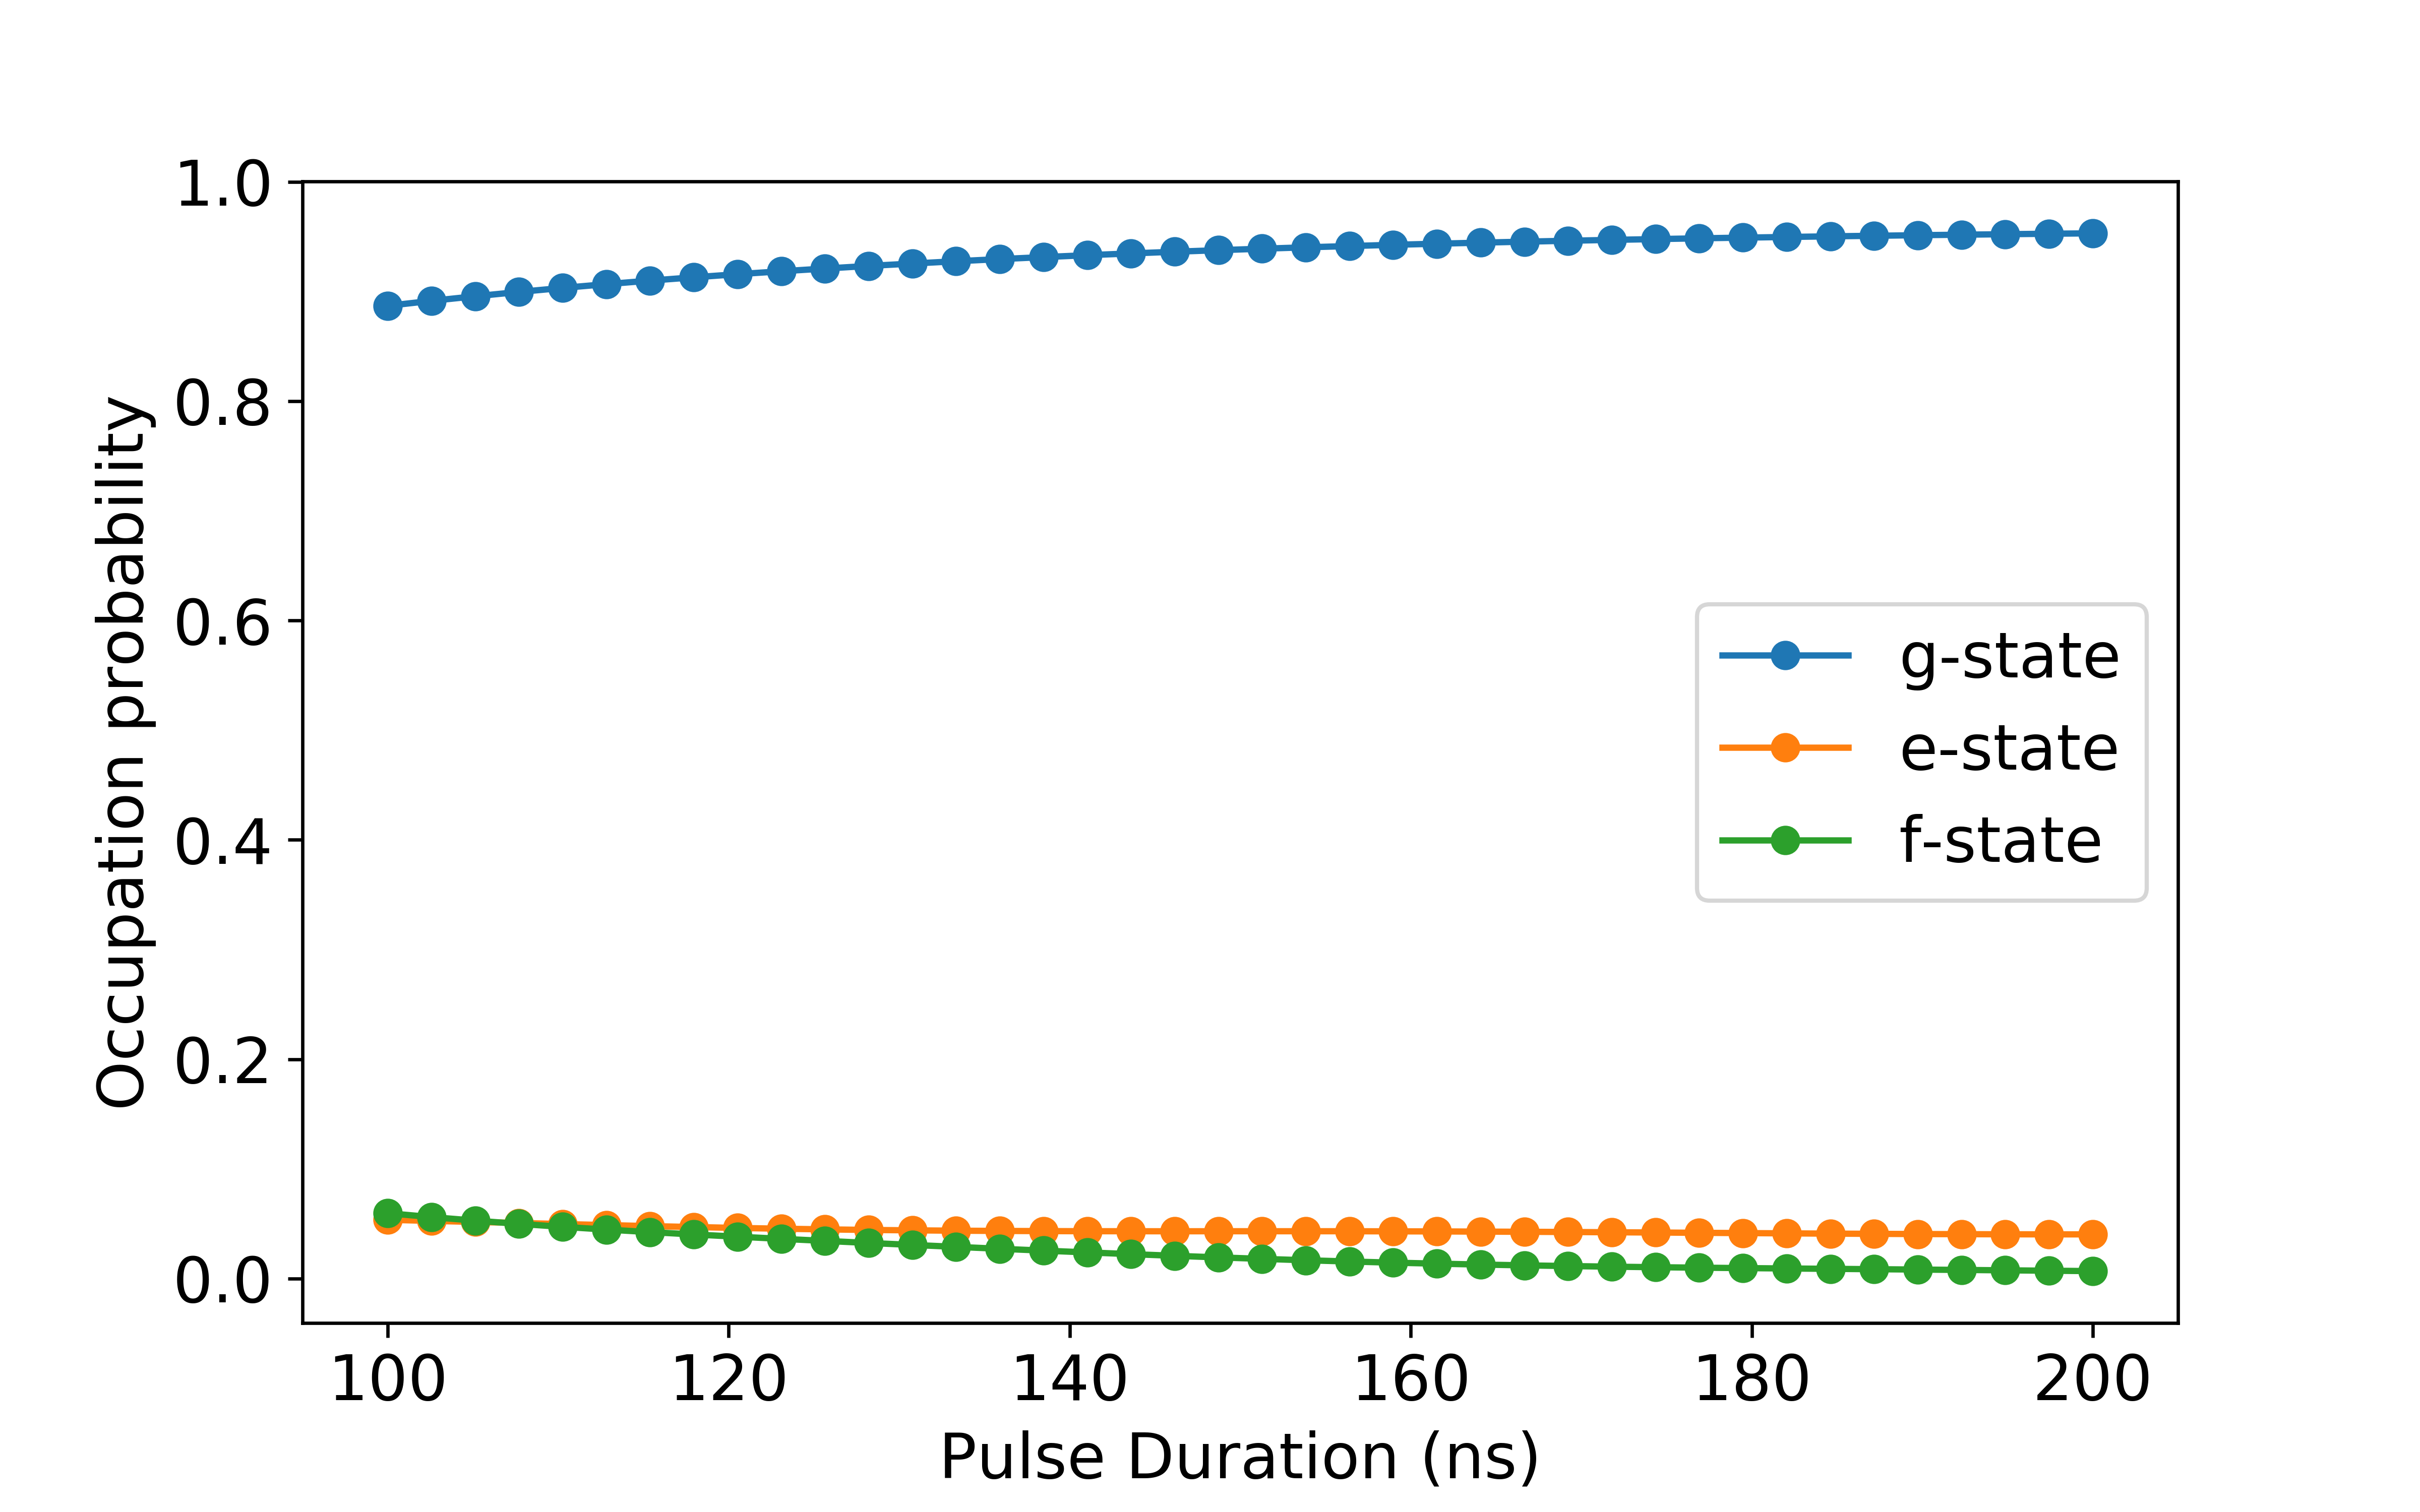
\includegraphics[width=0.6\textwidth]{pic/different_reset_schemes/gef_pops.png}
    \caption{The population of the states of the qubit.}
    \label{fig:tau_sweep_qubit_states}
\end{figure}

The prolonged application of driving pulse is forcing the population into qubit ground state, as depicted in Fig. \ref{fig:tau_sweep_qubit_states}. 




















\begin{figure}[h!]
    \centering
    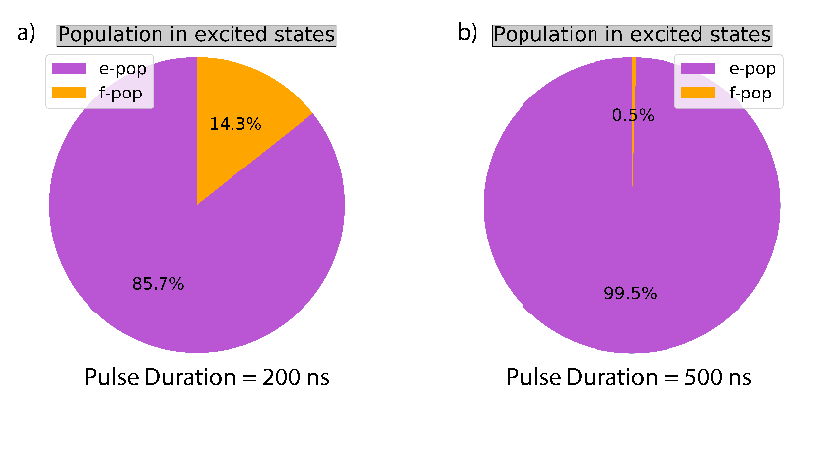
\includegraphics[width=0.6\textwidth]{pic/different_reset_schemes/dist_exc_tau_sweep.eps}
    \caption{The ratio of the population residing in $\ket{e}$ and $\ket{f}$ states for pulse duration of 200 and 500 ns. a) The overall population in excited states is The overall population in excited states is 5.6$\%$  b) The overall population in excited states is 2.5$\%$.}
    \label{fig:tau_sweep_qubit_states}
\end{figure}



























\subsection{Explanation of Functions}

\textcolor{blue}{This part could be moved in Gitlab not to overwhelm the report too much!}

\subsection{ Hamiltonian}
\textcolor{green}{This function calculates the time dependent Hamiltonian for given $\omega_{eg}$, $\omega_{read}$, $\omega_{reset}$, $\omega_{pump}$, $\alpha$, $g_1$, $g_2$, $\Omega_{d}$ (variable name as "drive rate"), $\tau$ (the length of the pulse) and $t$ (time duration of simulation), also for the simulation the  Hilbert spaces in which qubit, readout and reset mode live should be truncated. Thus, \emph{qubit trunc}, \emph{read trunc}, and \emph{reset trunc} are corresponding to the number of modes for qubit and cavities to be considered in the simulation. The Jupyter notebooks for the simulations will be made publicly available on GitHub \cite{OUR GITLAB}.
}

\subsection{Population}

In this function, the collapse operators are introduced, and QuTiP's "mesolve" function is utilized to solve the master equation corresponding to the system. This function returns the expectation value of the population of the qubit for a given time vector, $t$.







\section{Cavity-assisted quantum bath engineering}

\subsection{}